% Anonymous review manuscript. See ../REVISION_STATUS.md before submission.
% Conference template: full-paper-template.zip / LaTex+Package.rar, retrieved 2026-09-15.
\documentclass[runningheads]{llncs}
\usepackage[T1]{fontenc}
\usepackage{amsmath}
\usepackage{amssymb}
\usepackage{graphicx}
\usepackage{booktabs}
\usepackage{xurl}
\usepackage[hidelinks]{hyperref}
\urlstyle{rm}
\hypersetup{pdfauthor={},pdftitle={History-Conditioned Control under Unseen Actuator Faults: An Eight-Seed Evaluation},pdfsubject={Anonymous conference review manuscript},pdfkeywords={reinforcement learning, actuator faults, history conditioning, empirical evaluation}}
\newcommand{\rltwo}{RL\textsuperscript{2}}
\newcommand{\ReturnRows}{%
Action latency & 469.2 & 531.0 & 447.3 \\
Dead actuator & 1929.3 & 2059.4 & 2470.8 \\
Sign flip & 1126.3 & 1289.7 & 1309.0 \\
}

\newcommand{\EffectRows}{%
Action latency & $-61.8$ & $[-231.3, +141.6]$ & $+21.9$ & $[-73.6, +111.2]$ \\
Dead actuator & $-130.1$ & $[-354.3, +58.9]$ & $-541.4$ & $[-997.6, -201.0]$ \\
Sign flip & $-163.5$ & $[-303.4, -24.7]$ & $-182.8$ & $[-431.6, +3.8]$ \\
}

\begin{document}
\title{History-Conditioned Control under Unseen Actuator Faults: An Eight-Seed Evaluation}
\titlerunning{History-Conditioned Control under Unseen Actuator Faults}
\author{Anonymous Author(s)}
\authorrunning{Anonymous submission}
\institute{}
\maketitle

\begin{abstract}
History-conditioned policies can use past observations, actions, and rewards to respond to hidden changes in dynamics. Whether that capability improves control under an unseen actuator fault requires an explicit empirical test. We evaluate a transformer actor--critic trained on action scaling and action noise in HalfCheetah-v5. Eight independent training seeds are compared with the same checkpoints evaluated using a single observation token and with eight separately trained reactive baselines. Checkpoints are selected using validation perturbations from the training mechanisms; held-out tests contain action latency, a disabled actuator, or a sign reversal. Across 25 deterministic episodes per seed and condition, the primary latency history effect is $-61.8$ return units, with a 95\% seed-level bootstrap interval of $[-231.3,141.6]$. The corresponding advantage over the reactive baseline is $21.9$ with interval $[-73.6,111.2]$. Thus, positive history-enabled adaptation is not established for this configuration. A code and checkpoint audit identifies a material limitation: training uses 32-token windows while history-enabled inference can use 64 tokens, including positional embeddings outside the training window. These findings concern the evaluated implementation and do not establish an intrinsic disadvantage of memory. A separately documented TrackMania run illustrates the narrower evidence available from a single real-time deployment. The study provides reproducible result aggregation and identifies controls required for stronger adaptation claims.
\keywords{Reinforcement learning \and Actuator faults \and History conditioning \and Empirical evaluation \and Real-time control}
\end{abstract}

\section{Introduction}
An autonomous controller can encounter changes that are absent from its current observation: an actuator may respond late, lose effectiveness, or reverse direction. The same state and commanded action can then lead to different outcomes. A history of commands and their consequences may help a policy infer the active dynamics. This motivates memory-based reinforcement learning (RL), but the availability of history alone does not demonstrate that a learned policy adapts successfully.

In-context RL represents an adaptation process in the activations of a sequence model. The original \rltwo{} formulation conditions a recurrent policy on observations, actions, rewards, and termination signals~\cite{rl2}. More recent work demonstrates that carefully configured recurrent baselines~\cite{ni} and transformer agents~\cite{amago} can solve a variety of partially observed and meta-learning problems. Algorithm Distillation offers another route by learning from the training histories of an RL algorithm~\cite{ad}. These results motivate testing history-conditioned control under changed dynamics; they do not guarantee a benefit for a particular implementation, training distribution, or fault mechanism.

Two questions must be separated. First, does retaining a sequence improve the performance of a particular frozen policy relative to removing most of that sequence? Second, does that policy control the system better than a separately trained reactive controller? A positive answer to one question need not imply a positive answer to the other. A controller could depend on history yet remain less effective than a simpler baseline, or it could achieve robust returns without exploiting a long context. Evaluation design must also distinguish independent training runs from repeated episodes of a single trained agent~\cite{empirical}.

We examine these questions in a bounded HalfCheetah-v5 study. A compact transformer policy is trained using only scaling and additive-noise perturbations. Checkpoint selection uses different parameter ranges of those same mechanisms. The primary test introduces delayed actions, which require temporal reasoning and were excluded from both training and validation. Two secondary tests disable or reverse one actuator. We retain all eight training seeds and compare their paired evaluation returns with a single-token evaluation and an independently trained reactive baseline. We also audit the relationship between the implemented sequence protocol and its interpretation.

The contribution is an empirical evaluation of this configuration, rather than a claim of a new general-purpose RL algorithm. It comprises (i) a validation-selected, eight-seed comparison with explicit history and controller contrasts; (ii) a reproducible aggregation of 1,800 recorded evaluation episodes linked to checkpoint hashes; and (iii) an implementation audit that limits the interpretation of the observed history effect. A TrackMania deployment observation provides practical context, with a separate evidential status from the controlled benchmark. The resulting evidence does not establish positive adaptation to unseen action latency.

\subsection{Related Work and Design Context}
\paragraph{History and adaptation.}
Memory-based model-free RL is sensitive to architecture, context length, and optimization choices~\cite{ni}. AMAGO revisits off-policy in-context learning with transformers and long sequences~\cite{amago}; AMAGO-2 addresses multi-task optimization through objectives that reduce sensitivity to differences in return scale~\cite{amago2}. Our agent uses a much smaller, fixed configuration and a conventional regression-based critic objective. It neither reproduces the full AMAGO training recipe nor evaluates the breadth of tasks used in those studies. Unlike Algorithm Distillation~\cite{ad}, it learns directly from environmental reward and an auxiliary training-fault label rather than from a dataset of learning histories. Its context resets at each episode boundary; no across-episode adaptation is evaluated.

\paragraph{Off-policy continuous control.}
Soft Actor-Critic (SAC) combines off-policy learning with an entropy-regularized stochastic policy~\cite{sac}. REDQ uses an ensemble of critics and a random subset for target minimization~\cite{redq}. DroQ and CrossQ demonstrate that normalization and update scheduling can substantially affect efficiency~\cite{droq,crossq}. These methods motivate careful reporting of optimization details. Our benchmark uses a REDQ-style ensemble with LayerNorm critics. It does not implement the complete DroQ or CrossQ algorithm, and it does not compare against their published results.

\paragraph{Prior data and real-time interaction.}
RLPD shows how offline trajectories can support subsequent online learning when combined with appropriate off-policy design choices~\cite{rlpd}. DrQ-v2 demonstrates the importance of efficient visual learning and augmentation in continuous control~\cite{drqv2}. These findings motivate the use of demonstrations and image augmentation in the TrackMania case. TMRL provides a distributed framework and a real-time TrackMania environment~\cite{tmrl}. These features support real-time deployment. They also require choices about demonstration retention, observation timing, and asynchronous data collection that do not arise in a synchronous simulator. Our single-run observation cannot isolate their individual causal contributions.

\section{Method}
\subsection{Environment, Observation, and Fault Splits}
We use HalfCheetah-v5 through Gymnasium~\cite{gym}. It has a 17-dimensional state observation, six continuous action dimensions, and an episode horizon of 1,000 steps. A wrapper samples a hidden actuator perturbation at reset. Its mechanism and persistent parameters remain fixed within that episode; additive-noise realizations are sampled at each step. The policy receives the packed token
\begin{equation}
 x_t = [s_t, a_{t-1}^{\mathrm{cmd}}, r_{t-1}, d_{t-1}] \in \mathbb{R}^{25},
 \label{eq:token}
\end{equation}
where the preceding action is the commanded action before corruption. Previous-action, reward, and terminal fields are zero at reset. The terminal flag records environment termination, while a time-limit truncation ends collection without being treated as an absorbing terminal transition in the critic target.

The wrapper transforms $a_t^{\mathrm{cmd}}$ into an applied action and clips the result to the environment's action bounds. It returns the base environment reward after applying that action. Therefore, the reported return includes the effects of the transformation on both dynamics and the base reward calculation. It is neither normalized across conditions nor a success-rate measure. Fault identity is available to the auxiliary training loss but is excluded from the input token.

\begin{table}[t]
\caption{Perturbation splits. Scaling is sampled independently for each action dimension. The latency queue starts with zero actions.}
\label{tab:faults}
\centering\small
\begin{tabular}{@{}p{0.15\textwidth}p{0.22\textwidth}p{0.55\textwidth}@{}}
\toprule
Split & Mechanism & Sampling or transformation \\
\midrule
Training & Scaling / noise & Equal probability of either mechanism. Scale factors $u_j\sim U[0.5,1.5]$; or independent Gaussian noise with standard deviation $0.5$. \\
Validation & Scaling / noise & Equal probability of either mechanism. Scaling uses either $[0.2,0.5]$ or $[1.5,1.8]$, selected with equal probability per episode; noise standard deviation is $0.75$. \\
Primary test & Action latency & Delay $k$ sampled uniformly from $\{1,2,3,4,5\}$ steps; apply the command from $k$ steps earlier. \\
Secondary tests & Dead actuator; sign flip & Select one of six dimensions uniformly and either set its applied value to zero or multiply it by $-1$. Each condition is evaluated separately. \\
\bottomrule
\end{tabular}
\end{table}

Table~\ref{tab:faults} defines the splits. Delayed commands introduce a temporal mechanism excluded from training and validation. Disabling or reversing an actuator extrapolates the per-dimension scaling transformation to zero or a negative factor. Consequently, these two secondary conditions should not be presented as evidence of adaptation to entirely unrelated mechanisms. No demonstrations are used in this benchmark.

\subsection{Policies and Context Intervention}
The sequence agent embeds each token into a 64-dimensional representation using a multilayer perceptron, LayerNorm, and a GELU activation. Two causal transformer blocks each have two attention heads and a 128-unit feed-forward layer. Learned absolute positional embeddings have 128 available positions, and transformer dropout is $0.1$ during training. An eight-dimensional task embedding is obtained from the transformer output through a linear layer and ReLU. A seven-output classification head is trained with the wrapper's fault index; only scaling and noise labels occur in the training split. The auxiliary weight is $0.05$.

The Gaussian actor reads the transformer representation and task embedding. It uses two 128-unit hidden layers and a tanh-squashed action distribution. Ten critic heads receive the representation, task embedding, and action; each has two 256-unit hidden layers with LayerNorm. The actor receives detached representations, so its objective does not directly update the transformer trunk. Critic regression and the auxiliary classification loss train the shared representation. Neural-ODE components and split recurrent encoders are disabled in this benchmark.

Collection and evaluation with history use a queue of up to 64 packed tokens within each episode. At every action the sequence is processed afresh, and the actor uses the final output. The queue resets at episode boundaries. In the single-token intervention, the same trained agent clears its queue before each action and then processes the current packed token. The original implementation calls this mode \texttt{no\_history}; we use \emph{single-token} to make its information content explicit. Equation~\ref{eq:token} still supplies the previous command and reward. This intervention removes longer context but does not remove all temporal information.

The independently trained baseline is a feed-forward SAC/REDQ-style agent with a two-layer, 256-unit actor and ten two-layer, 256-unit LayerNorm critics. It receives the same 25-dimensional packed token and has no internal sequence state. We call it \emph{reactive} with respect to that token. It is not a state-only baseline. Its width and input processing differ from the transformer agent, so the comparison is a controller-level benchmark rather than a parameter-matched architecture ablation.

\subsection{Replay, Objectives, and Training Budget}
Transformer replay stores complete episodes and samples contiguous 32-token training windows. The first eight positions provide context; critic and actor losses use the remaining 24 positions. The auxiliary classification loss uses the final position. The reactive agent samples individual transitions. Both replay capacities are one million transitions and both batch sizes are 64, but a sequence batch contains many more supervised positions than a transition batch. Equal batch size therefore does not imply equal optimization work or equal exposure to replayed transitions.

For a next action sampled from the current policy, the critic target follows the REDQ-style construction
\begin{equation}
 y_t = r_t + \gamma(1-d_t)
 \left[\min_{j\in\mathcal{M}} Q_{\bar\theta_j}(f'_{t+1},a')
       -\alpha\log\pi_\phi(a'\mid f'_{t+1})\right],
 \label{eq:target}
\end{equation}
where $|\mathcal{M}|=2$ critics are sampled from the ensemble of ten and $f'_{t+1}$ denotes the next policy features. In the sequence agent, target features come from target copies of the trunk and task encoder. Critic losses are summed across the ten heads. The actor minimizes $\alpha\log\pi-Q$, using the minimum of critics 1 and 2, with entropy temperature learned separately. The target discount is $\gamma=0.99$.

Each run contains 100 iterations. An iteration collects four complete episodes, then performs 100 actor/temperature update cycles. Each cycle contains ten critic-ensemble updates followed by one actor and one temperature update. The archived manifest records 400,000 environment steps for every run, yielding 100,000 critic-ensemble updates and 10,000 actor updates under this loop. The ratio of critic-ensemble updates to newly collected environment steps is therefore $0.25$; the ratio of critic to actor updates is ten. Reporting the latter as an update-to-data ratio would be misleading. These counts do not equate the computational cost of the two architectures.

\begin{table}[t]
\caption{Shared optimization settings and evaluation schedule. Architecture-specific replay and context details appear in the text.}
\label{tab:settings}
\centering\small
\begin{tabular}{@{}ll@{}}
\toprule
Setting & Value \\
\midrule
Independent training seeds per architecture & 42--49 (eight runs) \\
Actor / critic / temperature learning rates & $3\times10^{-4}$ / $1.5\times10^{-4}$ / $3\times10^{-4}$ \\
Optimizer; gradient-norm clipping & Adam; 10 \\
Discount; target-network retention & $0.99$; $0.995$ \\
Target entropy; initial temperature & $-6$; $1$ \\
Replay capacity; batch size & $10^6$ transitions; 64 \\
Training iterations; episodes per iteration & 100; 4 \\
Validation interval; episodes per checkpoint & 10 iterations; 10 \\
Final episodes per seed, condition, and mode & 25 \\
\bottomrule
\end{tabular}
\end{table}

The saved environment records report Python 3.12.10, PyTorch 2.11.0 with a CUDA 12.8 build, Windows 11, and an NVIDIA GeForce RTX 5070 Laptop GPU. Historical Gymnasium and simulator package versions were not captured. The study therefore documents the recorded runtime without claiming an exact, fully pinned reproduction environment. Table~\ref{tab:settings} summarizes the principal settings.

\subsection{Checkpoint Selection and Final Evaluation}
Each run is validated every ten iterations using ten deterministic episodes from the validation split. A checkpoint is retained when its mean validation return improves. Validation environment seeds depend on the training seed and iteration, so candidate checkpoints do not share a fixed validation episode set; the finite validation sample introduces selection noise. The selection rule nevertheless avoids querying the held-out fault mechanisms. After training, the retained checkpoint is loaded and evaluated on all three test conditions without parameter updates.

For each condition and evaluation mode, episode $e\in\{0,\ldots,24\}$ uses environment seed $50000+100e$. The same seed schedule is used for both transformer modes and the reactive baseline, and is repeated across training seeds. Thus, initial states and sampled fault parameters are matched across policy comparisons. The retained context can alter the trajectory, but it cannot change the initial condition or the episode's persistent test fault. All recorded test episodes have length 1,000.

An earlier exploratory manuscript used held-out-fault performance for checkpoint selection. Its underlying three-seed records could not be reliably linked to the available experiment archive. We exclude its numerical results from this evaluation. The present protocol uses a different training budget and selection rule, so a difference from the exploratory account cannot be attributed solely to removing test-set selection. The available protocol file predates the recorded runs, but this is not evidence of public preregistration.

\subsection{Estimands, Uncertainty, and Evidence Audit}
Let $R_{i,c}^{H}$, $R_{i,c}^{S}$, and $R_{i,c}^{B}$ be the mean undiscounted episode returns for training seed $i$ and fault condition $c$, using history-enabled transformer inference, single-token transformer inference, and the reactive baseline, respectively. We compute
\begin{equation}
 G_{i,c}=R_{i,c}^{H}-R_{i,c}^{S},\qquad
 D_{i,c}=R_{i,c}^{H}-R_{i,c}^{B}.
 \label{eq:effects}
\end{equation}
$G$ measures the implemented context intervention on the same checkpoint. $D$ measures controller performance relative to the trained baseline. The primary question is whether the mean latency effect $\bar G_{\mathrm{latency}}$ is positive with an uncertainty interval entirely above zero. The two other fault conditions and all baseline contrasts provide additional descriptive evidence.

For each contrast, we resample the eight seed-level differences with replacement 2,000 times, using NumPy random seed 12345, and take the 2.5th and 97.5th percentiles of the resampled means. We retain all eight seeds. Episodes within a seed are averaged before resampling, avoiding treating repeated evaluation episodes as independent training replications~\cite{empirical}. The baseline contrast pairs runs by their designated seed labels; this pairs the experimental schedule, not identical network initializations. Intervals are pointwise and are not corrected for multiple comparisons. With eight training seeds, bootstrap tail estimates remain approximate. Because the test episode schedule is fixed, these intervals primarily describe training-seed variability conditional on that schedule, not uncertainty over every possible initial state and fault.

The analysis checks 1,200 transformer records ($8\times3\times2\times25$) and 600 reactive records ($8\times3\times25$). It verifies episode identifiers, pairing, validation-selected iteration, and the match between all 16 checkpoint file hashes and their recorded metadata. Tables are regenerated from the archived CSV returns, which were rounded to four decimal places. The source package includes these records and the deterministic aggregation script. Recomputing the statistics verifies their consistency with the archive; it does not independently rerun the environment or establish that every historical training detail was captured.

\section{Results}
\subsection{Primary Latency Comparison}
Table~\ref{tab:returns} reports mean returns, averaged equally across training seeds. Under delayed actions, mean return is $469.2$ with history, $531.0$ with a single token, and $447.3$ for the reactive baseline. The mean history effect is $-61.8$ with a 95\% interval of $[-231.3,141.6]$ (Table~\ref{tab:effects}). The interval includes zero and does not support a positive history effect. It also does not establish equivalence between the two modes.

\begin{table}[!htbp]
\caption{Held-out mean episode returns. Each entry averages eight training-seed means, each based on 25 deterministic episodes. These are returns, not percentages or success rates.}
\label{tab:returns}
\centering\small
\begin{tabular}{@{}lrrr@{}}
\toprule
Fault & History-enabled & Single-token & Reactive \\
\midrule
\ReturnRows
\bottomrule
\end{tabular}
\end{table}

The individual latency effects for seeds 42--49 are $-136.4$, $-319.9$, $517.8$, $-5.1$, $-315.1$, $-277.0$, $147.9$, and $-106.9$. Only two of eight are positive. This variation is visible in Fig.~\ref{fig:effects} and prevents a claim of consistently beneficial history. The mean advantage over the reactive controller is $21.9$ with interval $[-73.6,111.2]$. The recorded data therefore establish neither a positive history effect nor a clear controller-level advantage on the primary endpoint.

\begin{table}[!htbp]
\caption{Seed-level contrasts from Eq.~\ref{eq:effects}. Brackets are pointwise 95\% percentile bootstrap intervals over eight training seeds. Positive values favor history-enabled inference. Secondary intervals have no multiplicity correction.}
\label{tab:effects}
\centering\small
\begin{tabular}{@{}lrrrr@{}}
\toprule
Fault & Mean $G$ & 95\% CI for $G$ & Mean $D$ & 95\% CI for $D$ \\
\midrule
\EffectRows
\bottomrule
\end{tabular}
\end{table}

\begin{figure}[t]
\centering
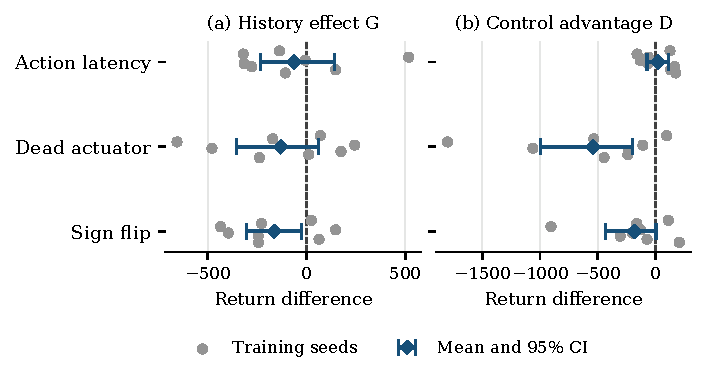
\includegraphics[width=\textwidth]{history_effects.pdf}
% Figure description: the two panels show all eight training-seed differences,
% with mean diamonds and bootstrap intervals; the latency G interval crosses zero.
\caption{Individual seed effects and their mean intervals. Gray points are the eight training-seed differences; blue diamonds and lines show the mean and its 95\% bootstrap interval. The dashed line denotes zero difference. The graphic is generated directly from the archived episode returns.}
\label{fig:effects}
\end{figure}

\subsection{Secondary Faults}
With a disabled actuator, the history-enabled, single-token, and reactive returns are $1929.3$, $2059.4$, and $2470.8$, respectively. The history effect is $-130.1$ with interval $[-354.3,58.9]$; four of eight seed effects are positive. The controller advantage is $-541.4$ with interval $[-997.6,-201.0]$, descriptively favoring the reactive baseline for this condition.

Sign reversal yields mean returns of $1126.3$ (history), $1289.7$ (single token), and $1309.0$ (reactive). The history effect is $-163.5$ with interval $[-303.4,-24.7]$; three of eight seed effects are positive. The controller advantage is $-182.8$ with interval $[-431.6,3.8]$. These secondary patterns are compatible with a history-related performance cost in this implementation, but the pointwise intervals do not establish a family of separately confirmed discoveries. Nor should the raw returns be used to rank the intrinsic severity of different fault types: they reflect this environment, fault sampling, and policy behavior together.

\subsection{Implementation Audit: Context-Length Mismatch}
The training window has 32 positions, whereas the history-enabled inference queue can contain 64. Training windows restart the learned absolute position indices at zero. Once an inference sequence grows beyond 32 tokens, it therefore uses positional embeddings that lie outside the training-window support. To check that this discrepancy is represented in the saved models, we compare checkpoint positional embeddings with a freshly initialized copy of the current implementation under the same training seed. In all eight checkpoints, positions 32--127 match that seeded initialization exactly, while positions 0--31 have changed. This is consistent with the inspected training loop and identifies a concrete mismatch between training and inference.

This audit does not measure how much of the return difference the mismatch causes. Single-token inference also changes the position of the final token, and its sequence length is outside the loss-bearing positions used during training. Both interventions therefore alter more than the amount of useful past information. The reported $G$ is an effect of these implemented inference modes; it is not an isolated causal estimate of the value of memory. A matched-context experiment is required before making that stronger inference.

\subsection{TrackMania Deployment Observation}
A separate real-time driving experiment used a reactive visual SAC controller within a TMRL-based pipeline~\cite{tmrl}. The original experiment notes describe four-frame image input, behavior-cloning initialization from 23 human demonstration laps (26,642 transitions), equal-proportion sampling from retained demonstration and online data, and random-shift image augmentation. These are recorded design details of the case, with motivations related to prior-data and visual-control methods~\cite{rlpd,drqv2}; the demonstration counts have not been independently reconciled with a complete exported dataset.

One experiment-tracker run can be linked to the manuscript's reported return and episode length. Its stored test summary is $279.7099914551$ return units and 1,372 environment steps. At the nominal 20 Hz collection schedule described in the experiment notes, this corresponds to 68.6 seconds of step-indexed duration; it is not an independently measured wall-clock lap time. The notes describe this episode as a track completion, but the available summary does not expose a separate finish flag or a repeated completion rate. We therefore report the numeric observation without treating it as verified reliable completion.

The tracked process ran for approximately 10 h 58 min and ended in a killed state. A saved summary is not necessarily a maximum-over-training statistic or the first successful episode. Two other development configurations in the exploratory manuscript could not be mapped confidently to their underlying runs and are excluded from quantitative comparisons. Consequently, this case does not estimate the causal benefit of demonstrations, establish a transformer-versus-CNN ranking, or demonstrate generalization to unseen tracks. The private tracker identifier is retained in the author audit record and omitted from the anonymous manuscript.

\section{Discussion}
\subsection{What the Results Establish}
The eight-seed study does not establish a positive latency history effect for the evaluated transformer configuration. Its primary interval spans both negative and positive effects, and six of eight seed differences are negative. The baseline comparison also remains uncertain. These are bounded statements about saved validation-selected checkpoints under a fixed evaluation schedule. They are compatible with the broader literature showing that memory can be useful when task structure and implementation support it~\cite{ni,amago}; they do not refute those results.

The implementation audit gives a reason to avoid interpreting the study as a clean test of memory capacity. Context length, position encoding, the intervention's input distribution, and the training objective all affect what information the policy can use. A change in performance after resetting context does not, by itself, demonstrate online system identification. A policy could exploit correlations in its recent inputs without identifying the fault, and an adverse positional shift could conceal a useful memory mechanism. Conversely, access to previous action and reward lets both the single-token mode and the reactive baseline exploit limited temporal information.

\subsection{Validity and Reproducibility Limits}
Several limits remain material. The benchmark contains one locomotion environment, eight training seeds per architecture, a fixed 400,000-step budget, and three fault conditions. There is no systematic hyperparameter search, context-length sweep, learned memory baseline other than the transformer, or parameter-matched architecture comparison. Although collection budgets and update-cycle counts match, sequence batches and transition batches differ in optimization work. The auxiliary fault classifier is not separately ablated, and its two observed training labels cannot establish identification of unseen fault mechanisms.

Checkpoint selection uses only validation mechanisms, but a ten-episode score and changing validation seeds can yield a noisy choice. Final evaluation uses the same finite episode schedule across all training seeds. A broader claim about a fault distribution requires additional held-out initial states and severities. The post hoc positional-embedding audit is a consistency check, not an additional control-performance experiment, and neither capped-context evaluation nor corrected training has been performed as part of this result set.

The saved checkpoint hashes, raw returns, and validation records support internal traceability. Historical source reconstruction is less complete: the recorded Git commit does not contain the benchmark scripts, which were untracked in the inspected workspace. The saved tracked-file diff consequently cannot establish the exact historical contents of those scripts. The source package preserves the currently inspected implementation separately and labels that limitation. Package versions for the historical environment are also incomplete. These gaps prevent a claim of exact end-to-end reproducibility, even though the reported aggregates can be regenerated from the supplied episode records.

The real-time case has still narrower external validity. It records one documented run on one track without matched repeated seeds, verified completion frequencies, or a complete provenance match for the alternative configurations. Demonstration availability, replay composition, policy architecture, augmentation, and entropy settings vary together in the development account. Attributing every outcome to replay or demonstrations would exceed the evidence. A reliable driving claim would require repeated policy-only executions with explicit finish detection, timing measurements, and track isolation.

\subsection{Implications for a Follow-up Evaluation}
The first priority is to align the context and positional support used during training and evaluation. A follow-up should either restrict all modes to supported positions or train with the intended deployment context, and document how sequence positions are handled in the single-token control. Evaluating a capped context on the existing checkpoints would be a useful post hoc diagnostic, while a fresh training protocol would be needed to assess a corrected agent without reusing the present held-out tests for selection.

The next comparison should include a state-only reactive controller, the present packed-token baseline, and a tuned recurrent baseline. Varying only context support within a fixed checkpoint would answer a different question from comparing fully retrained architectures; both should be labeled accordingly. Additional initial-state seeds, a fixed validation schedule, and separately defined fault severities would improve precision. These changes should be specified before inspecting the new test outcomes, following established empirical-design guidance~\cite{empirical}.

For the real-time application, retain immutable demonstration manifests, complete run histories, configuration snapshots, and explicit finish events. Compare replay composition and architecture under matched track, data, and training budgets. Report measured action latency and repeated completion rates alongside return. These controls would connect the simulator's fault-intervention questions to practical driving performance without assuming that a single high-return episode establishes reliability.

\section{Conclusion}
We evaluate history-conditioned control using eight transformer training seeds, eight reactive baselines, validation-selected checkpoints, and matched held-out fault episodes. On action latency, the mean history effect is $-61.8$. Its 95\% interval, $[-231.3,141.6]$, spans zero. Positive adaptation is therefore not established for this configuration. Secondary results likewise provide no consistent history-enabled improvement. The context-length and positional-support mismatch limits architectural interpretation, while incomplete historical source capture limits end-to-end reproducibility. A documented TrackMania run supplies a deployment observation but cannot establish reliable completion or a causal demonstration benefit. The resulting contribution is a traceable, qualified empirical result and a concrete account of the controls needed for a stronger adaptation study.

% Only the shared academic affiliation has been described by the authors.
% A complete competing-interests declaration still needs author confirmation.
% Do not insert a statement of no competing interests without confirmation.

\begin{samepage}
\section*{AI Usage Declaration}
Google Antigravity with a Gemini model was used to assist implementation of the research architecture and algorithms. OpenAI Codex was used to assist manuscript revision and restructuring, literature-source lookup, formatting, code inspection, and preparation of scripts that recompute statistics and plot recorded returns. The reported episode observations are taken from saved experiment records; the table values and quantitative figure are calculated from those records. Generative AI was not used to invent experimental observations. The authors remain responsible for the implementation, source verification, analysis, interpretation, and final manuscript.
\par\end{samepage}

\bibliographystyle{splncs04}
\bibliography{references}
\end{document}
